% CVPR 2026 Paper Template; see https://github.com/cvpr-org/author-kit

\documentclass[10pt,twocolumn,letterpaper]{article}

%%%%%%%%% PAPER TYPE  - PLEASE UPDATE FOR FINAL VERSION
\usepackage{cvpr}              % To produce the CAMERA-READY version

\usepackage{microtype}
\usepackage{multirow}

\definecolor{cvprblue}{rgb}{0.21,0.49,0.74}
\usepackage[pagebackref,breaklinks,colorlinks,allcolors=cvprblue]{hyperref}

%%%%%%%%% PAPER ID  - PLEASE UPDATE
\def\paperID{*****} % *** Enter the Paper ID here
\def\confName{CVPR}
\def\confYear{2026}

\newcommand{\pmstd}[1]{{\scriptsize$\pm$#1}}
\newcommand{\code}[1]{\texttt{\small #1}}

%%%%%%%%% TITLE - PLEASE UPDATE
\title{Assignment 1: Self-Supervised Learning with SimSiam on STL-10}

%%%%%%%%% AUTHORS - PLEASE UPDATE
\author{B125808026 TAI, WEI-HSUAN}

\begin{document}
\maketitle

%%%%%%%%% ABSTRACT
\begin{abstract}
We re-implement SimSiam~\cite{chen2021simsiam} with a ResNet-18 backbone and pretrain it on the 100k unlabeled images of STL-10.
With only 1,000 labeled images, a linear probe on the frozen SimSiam encoder reaches $80.98\pm0.35\%$ test accuracy (200 epochs, 3 pretraining seeds), while the same network trained from scratch reaches only $55.66\pm0.93\%$ even with a tuned batch size and lr.
We also reproduce the complete collapse reported in the original paper: removing either the stop-gradient or the predictor drops the linear probe to exactly chance level (10.00\%).
As a new ablation, we remove one family of augmentations at a time. Without cropping, SimSiam suffers \emph{dimensional collapse}: the backbone's effective rank falls from 318 to 6.7, and accuracy \emph{drops} with longer training.
Replacing the crop shows that the views must \emph{differ}: one crop shared by both views is as bad as none, independent random masking recovers two thirds of the gap, and permuted image tiles, which a CNN with global pooling easily ignores, barely help. Each pretrained model becomes invariant to exactly the transformation its views differ by, and only the crop's part-to-whole rescaling yields features that classify well.
\end{abstract}

%%%%%%%%% BODY TEXT
\section{Introduction}
\label{sec:intro}

SimSiam~\cite{chen2021simsiam} is one of the simplest self-supervised methods. It trains a Siamese network to make the representations of two augmented views of an image agree, and uses no negative pairs, no large batches and no momentum encoder.
Contrastive methods such as SimCLR~\cite{chen2020simclr} rely on negatives to avoid the constant solution, BYOL~\cite{grill2020byol} on a momentum encoder; SimSiam claims that a stop-gradient and a predictor alone suffice.

Without negatives, the difference between the two augmented views is SimSiam's \emph{only} learning signal.
SimCLR~\cite{chen2020simclr} found crop plus color the most important augmentation pair for contrastive learning, and InfoMin~\cite{tian2020infomin} argues that good views should share task-relevant information and differ in everything else.
The SimSiam paper, however, ablates the architecture and the loss but not the augmentations that create this signal.
In this report we re-implement SimSiam on STL-10~\cite{coates2011stl10} and study both sides.
We (i) show that SimSiam pretraining on 100k unlabeled images beats a tuned from-scratch baseline by 25.3 points with 1,000 labels (\cref{sec:exp_cls});
(ii) reproduce the complete collapse caused by removing the stop-gradient or the predictor (\cref{sec:exp_arch});
(iii) show that without cropping SimSiam suffers \emph{dimensional collapse} that worsens with training and that neither the loss nor the output std detects (\cref{sec:exp_aug}); and
(iv) decompose the crop and find that what matters is a content difference between the two views, not data diversity, and that each model learns exactly the invariance its views demand (\cref{sec:exp_crop}).

%-------------------------------------------------------------------------
\section{Environment and Codebase}
\label{sec:env}

All experiments ran on one NVIDIA GeForce RTX 5070 Ti (16\,GB, driver 570.211.01, CUDA 12.8) with Python 3.10.21, PyTorch 2.8.0 and torchvision 0.23.0 (\cref{fig:env}).
The code extends the course starter code.
\code{model.py} holds SimSiam and its loss, with \code{stop\_grad} and \code{predictor} flags for the ablations; \code{data.py} the STL-10 loaders, validation split and two-view augmentation with an \code{aug} option (\cref{sec:method});
\code{pretrain.py} logs loss, kNN accuracy and output std every epoch; \code{linear\_probe.py} trains a linear (or BN) probe on the frozen backbone and \code{sft.py} the same ResNet-18 from scratch.
\code{analyze\_rank.py} (erank), \code{eval\_probes.py} (AUROC/F1), \code{stats\_tests.py}, \code{analyze\_crop\_decomp.py} (tests) and \code{analyze\_invariance.py} do the analysis, and \code{run\_*.sh} drive all experiments.

\begin{figure}[t]
\centering
\includegraphics[width=0.5\linewidth]{figures/screenshot.png}
\caption{Experimental environment (\code{nvidia-smi}).}
\label{fig:env}
\end{figure}

%-------------------------------------------------------------------------
\section{Method}
\label{sec:method}

\subsection{SimSiam}
Given an image $x$, two random augmentations produce views $x_1$ and $x_2$.
An encoder $f$, consisting of a backbone and a projection MLP, maps each view to $z_i=f(x_i)$, and a prediction MLP $h$ maps it to $p_i=h(z_i)$.
With the negative cosine similarity $\mathcal{D}(p,z)=-\frac{p}{\|p\|_2}\cdot\frac{z}{\|z\|_2}$, the symmetric loss is
\begin{equation}
\mathcal{L}=\tfrac12\mathcal{D}(p_1,\text{sg}(z_2))+\tfrac12\mathcal{D}(p_2,\text{sg}(z_1)),
\label{eq:loss}
\end{equation}
where $\text{sg}(\cdot)$ is the stop-gradient. The minimum of $\mathcal{L}$ is $-1$.

We use a ResNet-18 backbone~\cite{he2016resnet} with its fc layer removed (512-d output), a 3-layer projection MLP ($512\!\to\!2048\!\to\!2048\!\to\!2048$, BN~\cite{ioffe2015bn} on every layer) and a bottleneck prediction MLP ($2048\!\to\!512\!\to\!2048$).

\subsection{Ablations}
\paragraph{Architecture.}
Following Sec.~4.1--4.2 of the original paper, we (a) remove the stop-gradient so that gradients flow through both branches, and (b) replace the predictor $h$ with the identity.

\paragraph{Augmentation.}
The original paper's EM-like hypothesis (Sec.~5) views SimSiam as approximately solving
\begin{equation}
\min_\theta\; \mathbb{E}_{x,\mathcal{T}}\bigl\|f_\theta(\mathcal{T}(x))-\eta_x\bigr\|^2,
\label{eq:em}
\end{equation}
where $f_\theta$ is the encoder and $\eta_x$ is the expected representation of $x$ over augmentations $\mathcal{T}$.
If the augmentations are too weak, this expectation becomes trivial.
To test this, we remove one family of augmentations at a time:
\textbf{no\_color} drops color jitter and grayscale, and \textbf{no\_crop} drops RandomResizedCrop, so that both views show the full image and differ only in flip and color.

\paragraph{Decomposing the crop.}
A crop shows only \emph{part} of the content, \emph{rescales and shifts} it, makes the two views differ and adds diversity across epochs. To separate these factors we replace it (keeping flip and color) with:
\textbf{crop\_in\_place} keeps a RandomResizedCrop-style region at its original position and scale and fills the rest with the dataset mean (partial content only);
\textbf{zoom\_out} shrinks the whole image to area fraction $a$ (crop-like aspect ratio) and pastes it at a random position on a mean-filled canvas (rescaling and shifting only);
\textbf{mask} keeps a random fraction $a$ of the 36 $16\!\times\!16$ patches and fills the rest with the mean (partial content, scattered, no rescaling);
\textbf{same\_crop} applies one random crop to \emph{both} views, so the data diversity matches the baseline but the views no longer differ in crop;
\textbf{shuffle} cuts each view into $2\!\times\!2$ tiles and permutes them independently (same content, different layout), and \textbf{shuffle\_shared} uses one permutation for both views (same seams, no layout difference) as its control.
In crop\_in\_place, zoom\_out and mask, $a\sim U(0.2,1)$ as in the crop, drawn independently for each view.

\subsection{Measuring Collapse}
\emph{Complete collapse} maps every input to one vector; in \emph{dimensional collapse}~\cite{hua2021feature,jing2022dimensional} the embeddings stay spread out but occupy a low-dimensional subspace.
The std of the $\ell_2$-normalized output ($1/\sqrt{d}$ when spread over the sphere, $0$ under complete collapse) detects only the former, so we also measure the effective rank (erank)~\cite{roy2007erank}, which RankMe~\cite{garrido2023rankme} showed predicts downstream performance without labels.
With $\sigma_k$ the singular values of the centered, $\ell_2$-normalized features of the 8,000 test images,
\begin{equation}
\text{erank}=\exp\Bigl(-\sum_k p_k\log p_k\Bigr),\quad p_k=\frac{\sigma_k}{\sum_j\sigma_j}.
\end{equation}
We focus on the 512-d backbone feature, the probe's input.

%-------------------------------------------------------------------------
\section{Experimental Setup}
\label{sec:setup}

\paragraph{Dataset.}
We use STL-10~\cite{coates2011stl10} at $96\times96$. Pretraining uses the 100k unlabeled images.
Classifiers train on the official fold~0 (1,000 images). Validation uses 500 held-out, label-balanced training images, and testing uses all 8,000 test images.

\paragraph{Pretraining.}
Following the original paper's CIFAR setting, we use SGD (momentum 0.9, weight decay $5\!\times\!10^{-4}$), batch size 512, $\text{lr}=0.03\times512/256$, a 10-epoch warmup and cosine decay. The augmentation is RandomResizedCrop (scale 0.2--1), horizontal flip, color jitter $(0.4,0.4,0.4,0.1)$ with $p{=}0.8$, and grayscale with $p{=}0.2$, without the Gaussian blur of its ImageNet setting. As in the paper, the predictor's lr is not decayed.
A kNN monitor~\cite{wu2018instance} ($k{=}200$, $\tau{=}0.1$) uses fold~0 as the memory bank and evaluates on the validation images after every epoch.

\paragraph{Evaluation.}
The \emph{linear probe} trains a linear layer on the frozen backbone with SGD (lr 30 as in MoCo~\cite{he2020moco}, no weight decay) for 50 epochs. The \emph{BN probe} adds a parameter-free BN before the linear layer as in MAE~\cite{he2022mae}, with lr chosen on validation.
The from-scratch baseline (\emph{SFT}) trains the whole ResNet-18 with the pretraining optimizer settings (batch 512, about 2 steps per epoch) for 50 epochs; a \emph{tuned SFT} uses batch 64 for 100 epochs with lr chosen on validation.
Both train with RandomResizedCrop (scale 0.08--1) and horizontal flip.
The pretrained encoder is always the final-epoch checkpoint; for the classifier we test the \emph{probe/SFT epoch} with the best validation accuracy.

\paragraph{Statistics.}
For the 200-epoch comparisons we pretrain with seeds 123/456/789, and linear-probe each model with 5 finetuning seeds (12/34/56/78/90).
The \emph{pretraining seed} is the unit of replication: we report the mean $\pm$ std over the 3 per-model means and compare settings with two-sided Welch $t$-tests~\cite{welch1947}.
We also compute macro one-vs-rest AUROC and macro F1 for every probe, and check every comparison under all three metrics with Holm correction~\cite{holm1979} (one family of 25 tests per metric).

%-------------------------------------------------------------------------
\section{Experiments}
\label{sec:exp}

The original paper uses ImageNet and ResNet-50, so we compare only qualitative trends.

\begin{figure*}[t]
\centering
\begin{minipage}{0.495\linewidth}\centering
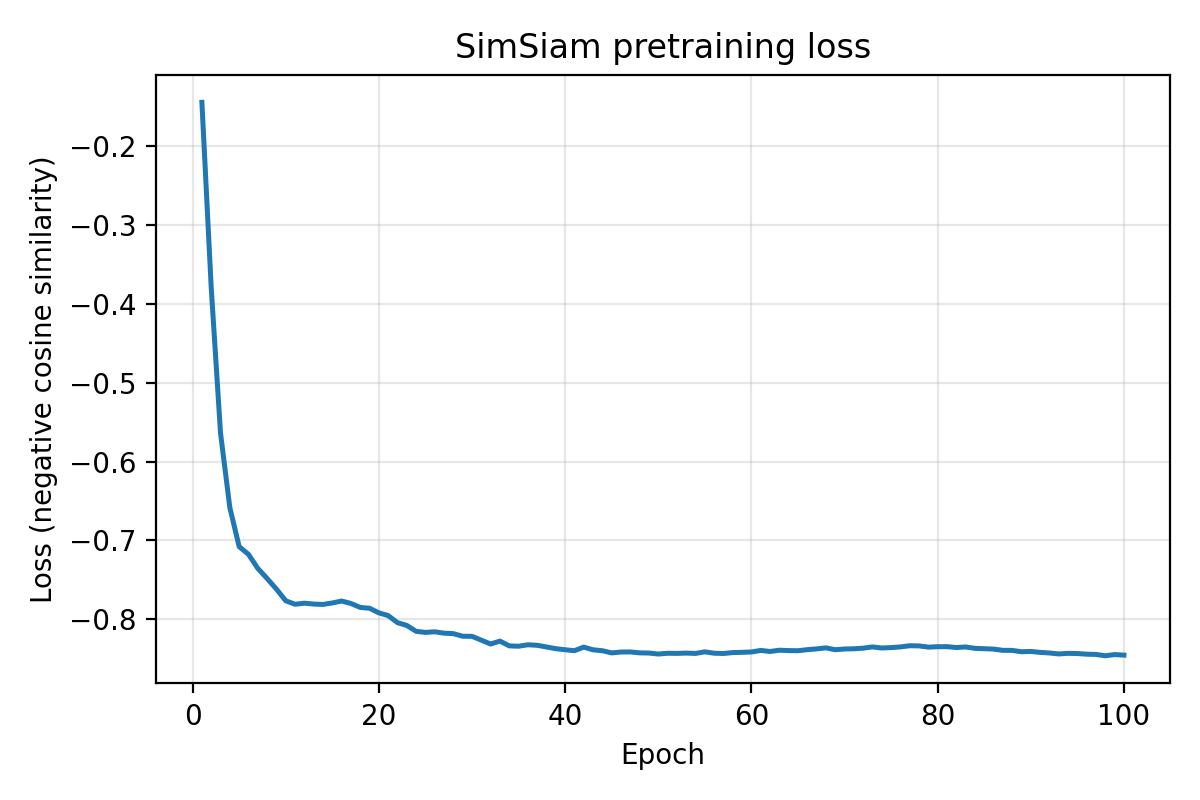
\includegraphics[width=0.49\linewidth]{figures/pretrain_loss.png}\hfill
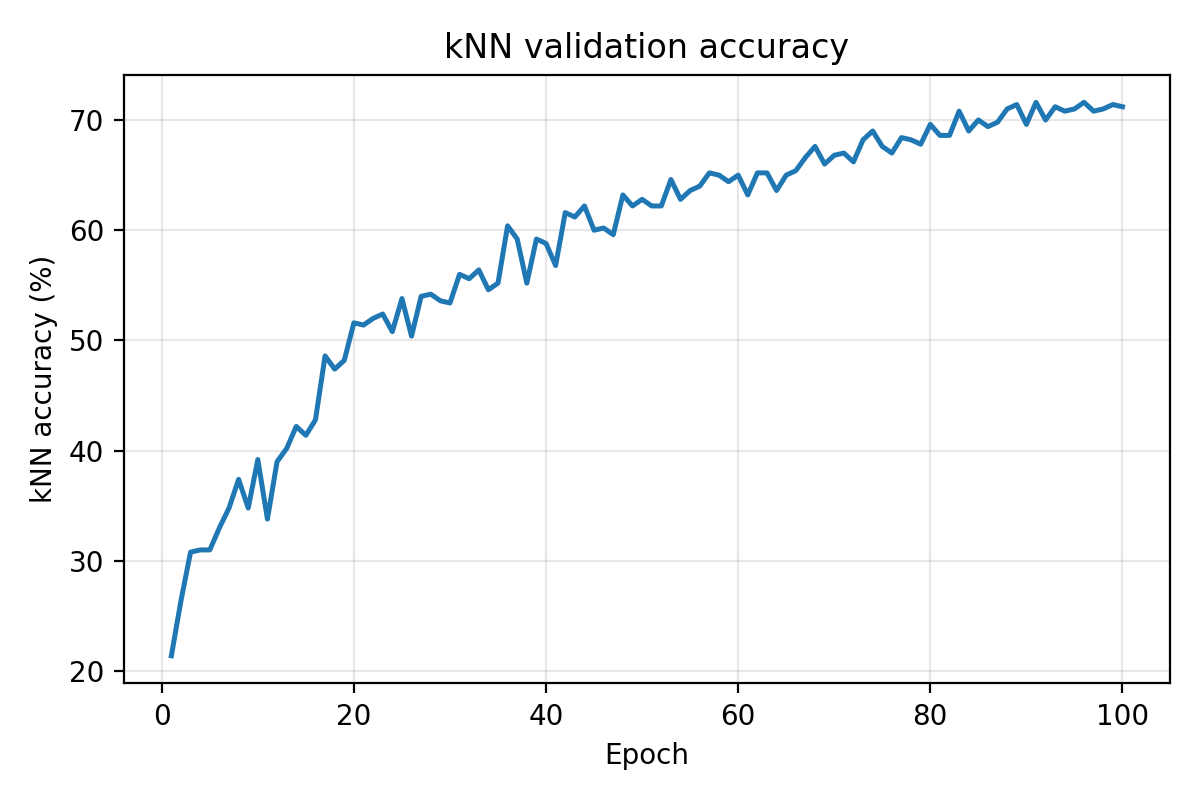
\includegraphics[width=0.49\linewidth]{figures/pretrain_knn.png}
\caption{SimSiam pretraining for 100 epochs: training loss (left) and kNN validation accuracy (right).}
\label{fig:pretrain}
\end{minipage}\hfill
\begin{minipage}{0.495\linewidth}\centering
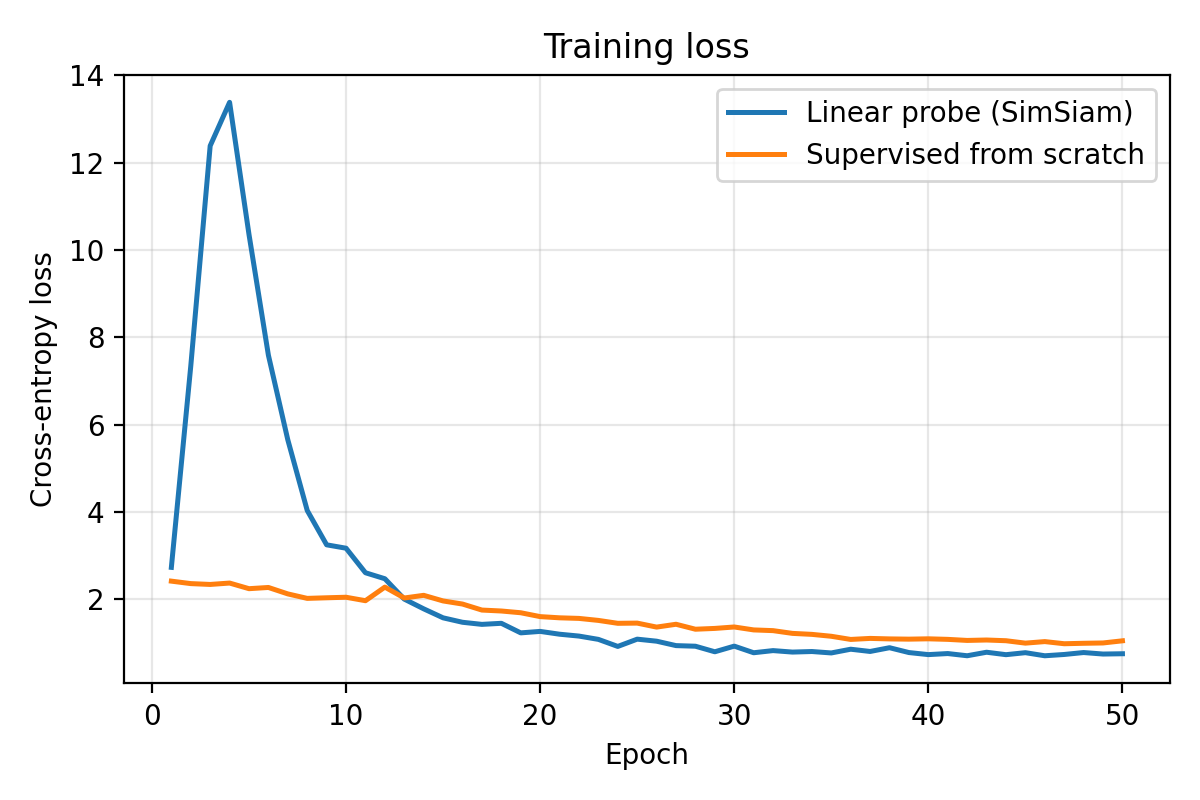
\includegraphics[width=0.49\linewidth]{figures/classify_loss.png}\hfill
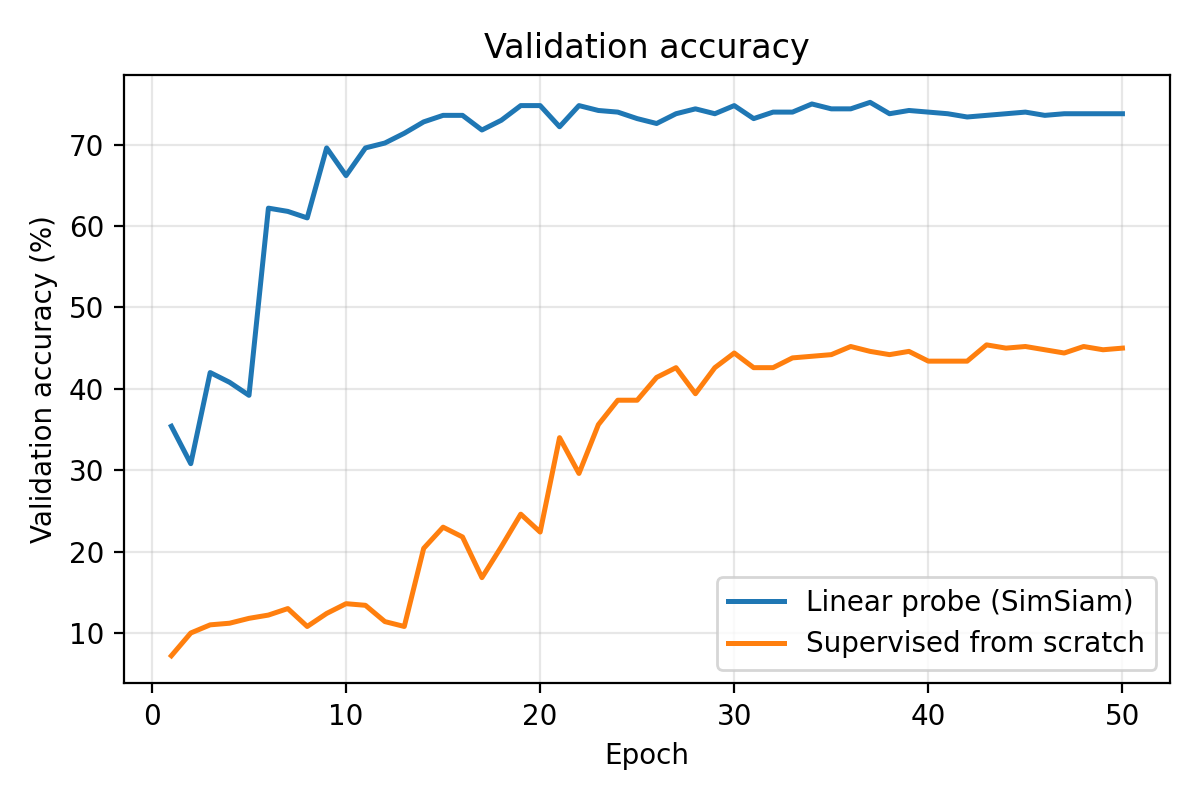
\includegraphics[width=0.49\linewidth]{figures/classify_val_acc.png}
\caption{Linear probe on the frozen 100-epoch encoder vs.\ SFT on the 1,000 fold-0 images: training loss (left) and validation accuracy (right).}
\label{fig:cls}
\end{minipage}
\end{figure*}

\subsection{SimSiam Pretraining}
\label{sec:exp_pretrain}



\Cref{fig:pretrain} shows a 100-epoch pretraining run.
The loss falls to about $-0.78$ during the 10-epoch warmup and ends at $-0.848$; the kNN accuracy rises steadily to 73.4\%.
The std of the normalized projector output ends at $0.02195$, close to $1/\sqrt{2048}=0.02210$, so the model has not collapsed.

Between epochs 50 and 80 the loss stays flat and even rises slightly ($-0.843\rightarrow-0.837$), while the kNN accuracy climbs from 60.6\% to about 70\%: the loss measures view agreement, not feature quality (\cref{sec:exp_aug}).

\subsection{Classification with and without Pretraining}
\label{sec:exp_cls}



\begin{table}[t]
\centering
\small
\setlength\tabcolsep{4pt}
\begin{tabular}{lccc}
\toprule
Method & Pretrain & Test acc.\ (\%) & $n$ \\
\midrule
SFT from scratch & -- & 47.74\pmstd{1.17} & 5 ft.\ seeds \\
SFT, tuned$^\ddagger$ & -- & 55.66\pmstd{0.93} & 5 ft.\ seeds \\
Linear probe & 100 ep & 75.80 & 1 run \\
Linear probe & 200 ep & \textbf{80.98}\pmstd{0.35} & 3 pt.\ seeds \\
Linear probe & 1000 ep & \textbf{86.74}\pmstd{0.23} & 1 run$^\dagger$ \\
\bottomrule
\end{tabular}
\caption{Test accuracy with 1,000 labeled images. $^\dagger$One pretraining run, so $\pm$ covers finetuning seeds only. $^\ddagger$Batch 64, 100 epochs, lr picked on validation from $\{0.03,0.1,0.3\}$.}
\label{tab:cls}
\end{table}

Both classifiers use the same ResNet-18 and the same 1,000 labeled images (\cref{fig:cls}, \cref{tab:cls}).
The linear probe passes 70\% validation accuracy around epoch 10, while SFT stays near chance for 13 epochs and plateaus around 45\%.
After 200 epochs of pretraining, the linear probe beats SFT by 33.2 points, and still by \textbf{25.3 points} (95\% CI 24.2--26.5, Welch $p{=}10^{-8}$) when SFT uses batch 64 (16 steps per epoch) and an lr tuned on validation.

Training longer does not close the gap either: at batch 512, SFT saturates at about 49--50\% (200 epochs: training loss 0.24, so it overfits), and a 200-epoch linear probe adds only $+0.8$ points over 50 epochs.
SimSiam therefore learns from the 100k unlabeled images what 1,000 labels alone cannot teach.
Longer pretraining keeps helping with diminishing returns (75.8, 81.0 and 86.7\% after 100, 200 and 1000 epochs), as in Tab.~4 of the original paper; in the 1000-epoch run loss and kNN accuracy plateau while the LR is above half its peak, and snapshot probes rise from 80 to 87\% only as it anneals.

\begin{figure}[t]
\centering
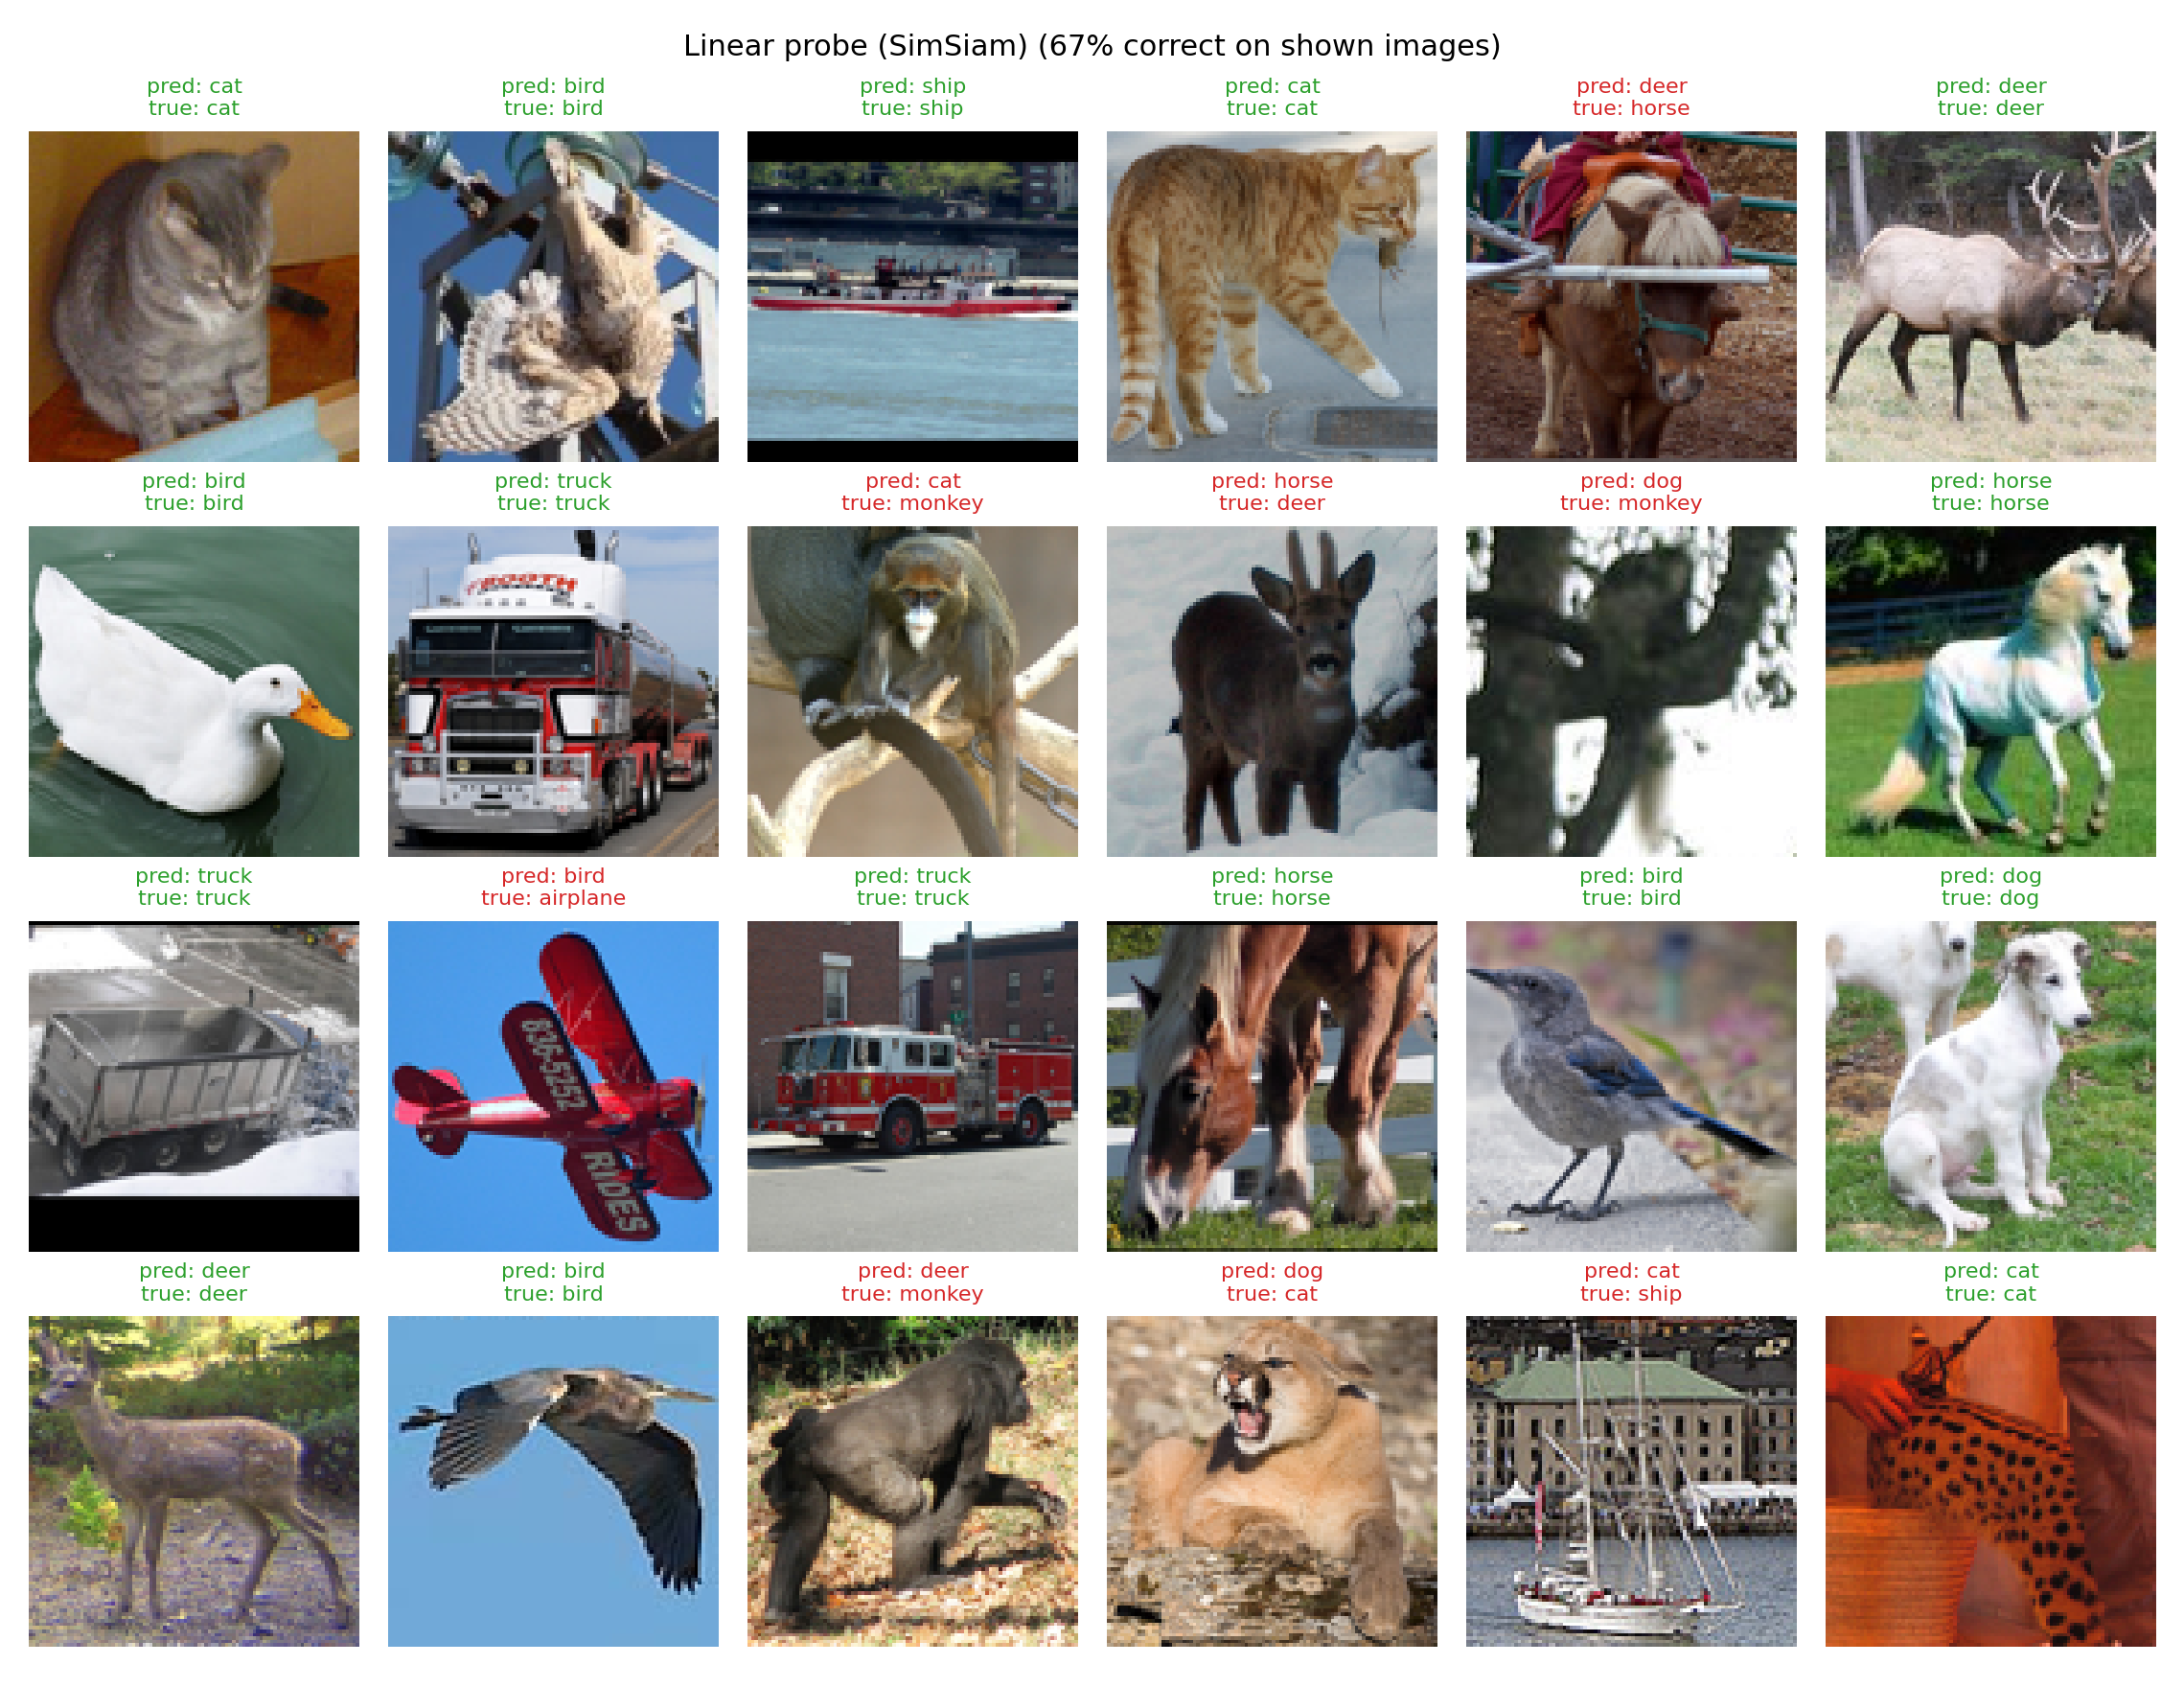
\includegraphics[width=0.56\linewidth]{figures/predictions_linear_probe.png}\hfill
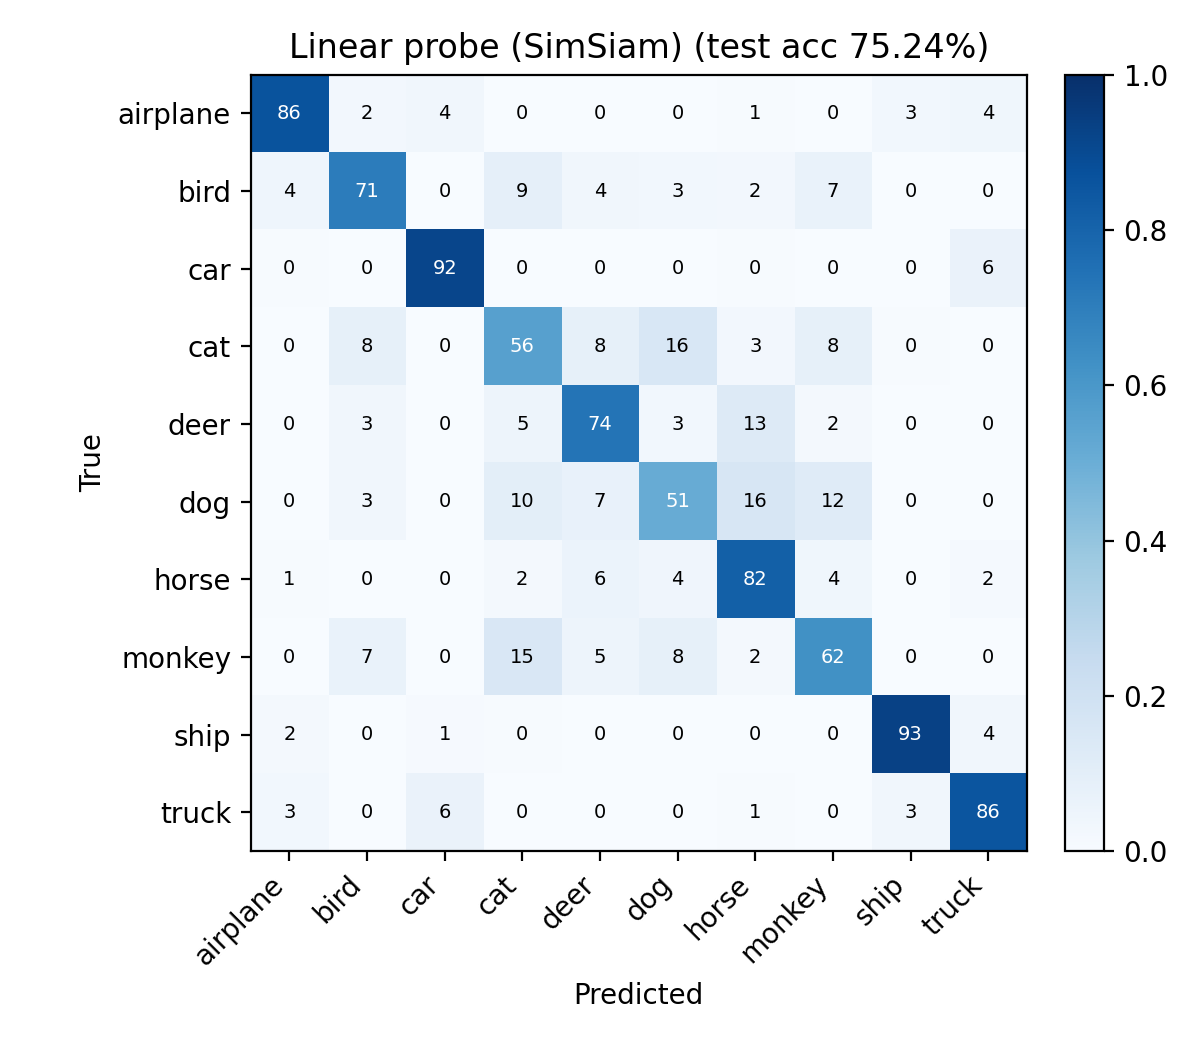
\includegraphics[width=0.43\linewidth]{figures/confusion_linear_probe.png}
\caption{Linear probe on random test images (left; green: correct, red: wrong) and its confusion matrix on all 8,000 test images (right). Errors concentrate among animal classes.}
\label{fig:pred}
\end{figure}

\paragraph{Error analysis.}
Errors are mostly between similar animals (cat$\leftrightarrow$dog, dog$\leftrightarrow$horse, deer$\leftrightarrow$horse; \cref{fig:pred}).
Vehicles (car, ship, truck, airplane) reach 86--93\% per-class accuracy.

\subsection{Ablation: Stop-Gradient and Predictor}
\label{sec:exp_arch}

\begin{figure*}[t]
\centering
\includegraphics[width=0.325\linewidth]{figures/e200_arch_pretrain_loss.png}\hfill
\includegraphics[width=0.325\linewidth]{figures/e200_arch_pretrain_std.png}\hfill
\includegraphics[width=0.325\linewidth]{figures/e200_arch_pretrain_knn.png}
\caption{Ablating the stop-gradient and the predictor (200 epochs): training loss, std of the $\ell_2$-normalized output (dashed: $1/\sqrt{d}$) and kNN accuracy. Both ablations collapse.}
\label{fig:arch}
\end{figure*}

\begin{table}[t]
\centering
\small
\setlength\tabcolsep{4pt}
\begin{tabular}{lcccc}
\toprule
Setting & Loss & Std & kNN & Lin.\ probe \\
\midrule
Baseline & $-0.908$ & 0.021 & 77.6 & 81.35 \\
w/o stop-grad & $-1.000$ & 0 & 10.0 & 10.00 \\
w/o predictor & $-1.000$ & 0 & 13.2 & 10.00 \\
\bottomrule
\end{tabular}
\caption{Architecture ablations after 200 epochs (final-epoch values; one unseeded run each, so the baseline differs slightly from \cref{tab:aug}).}
\label{tab:arch}
\end{table}

Both variants reproduce the collapse reported in the original paper (\cref{fig:arch}, \cref{tab:arch}).
Within a few epochs the loss reaches its minimum of $-1$ and the output std drops toward 0, so every image is mapped to the same vector.
After 200 epochs the linear probe scores \emph{exactly} 10.00\% with training loss $\ln 10 = 2.303$, which is chance level for 10 classes. The original paper's 0.1\% is the same result for ImageNet's 1000 classes.
After 100 epochs the probes still reach about 15\%, because the backbone has not fully collapsed yet.

The two ablations produce nearly the same curves, as the original paper's analysis predicts: without a predictor, the gradient of \cref{eq:loss} has the direction of that of $\mathcal{D}(z_1,z_2)$, so removing the predictor in effect also removes the stop-gradient.
The asymmetry from both components is required, in line with DirectPred~\cite{tian2021directpred}; collapse is deterministic, so one run per variant suffices.

\subsection{Ablation: Augmentation}
\label{sec:exp_aug}

\begin{table}[t]
\centering
\small
\setlength\tabcolsep{3pt}
\begin{tabular}{lcccc}
\toprule
Setting & Loss & kNN & Lin.\ probe & BN probe \\
\midrule
Baseline & $-0.909$ & 78.1 & \textbf{80.98}\pmstd{0.35} & \textbf{81.40}\pmstd{1.20} \\
w/o color & $-0.958$ & 44.9 & 50.36\pmstd{1.17} & 52.28\pmstd{1.25} \\
w/o crop & $-0.995$ & 19.3 & 17.50\pmstd{2.19} & 24.78\pmstd{1.54} \\
\bottomrule
\end{tabular}
\caption{Augmentation ablation, 200 epochs, mean (\pmstd{std}) over 3 pretraining seeds. Loss and kNN are final-epoch values averaged over seeds.}
\label{tab:aug}
\end{table}

\begin{figure*}[t]
\centering
\includegraphics[width=0.31\linewidth]{figures/e200_aug_pretrain_knn.png}\hfill
\includegraphics[width=0.67\linewidth]{figures/rank_bars.png}
\caption{Left: kNN accuracy during augmentation-ablation pretraining (one representative 200-epoch run each). Right: effective rank of test-set embeddings for the backbone features and projector output $z$ after 100 epochs (light) and 200 epochs (dark); bars are means and dots individual pretraining seeds. ``point'' means all images map to one point (relative variance $<10^{-4}$), so no rank is defined.}
\label{fig:aug}
\end{figure*}

\paragraph{Lower loss, worse representation.}
Both variants reach a \emph{lower} loss than the baseline, because the views are easier to align, yet their accuracy is far lower (\cref{tab:aug}).
With the same probe and $n{=}3$ on both sides, removing color costs 30.6 points ($p{=}1.8\!\times\!10^{-4}$), removing crop costs 63.5 points ($p{=}3.0\!\times\!10^{-4}$), and no\_crop is 32.9 points below no\_color ($p{=}1.6\!\times\!10^{-4}$).
The standard probe underestimates no\_crop (below), but the BN probe gives the same ordering (81.4, 52.3, 24.8; all pairs $p_\text{Holm}<10^{-3}$).
Cropping is therefore the more important augmentation. This agrees with SimCLR~\cite{chen2020simclr}, but the drop is larger here: without negatives, a too-easy view pair leaves no other signal to learn from.

\paragraph{The standard probe fails on no\_crop.}
With lr 30, the linear probe on no\_crop's tiny-variance features never gets below training loss $\ln 10$, even with 200 epochs.
The BN probe standardizes them (validation picks lr 1.0, vs.\ 0.03 for the baseline) and raises no\_crop to 24.78\% ($+7.27$, paired $p{=}0.003$), still 57 points below the baseline under the same probe; we use it for no\_crop below.

\paragraph{no\_crop gets worse with more training.}
no\_color improves from 100 to 200 epochs ($43.9\rightarrow50.4$), but no\_crop moves the other way.
With 3 seeded 100-epoch runs and the BN probe, its accuracy drops from $38.17\pm2.39$ to $24.78\pm1.54$ (Welch $t{=}8.18$, df 3.4, $p{=}0.0023$; 95\% CI of the change $[-18.3,-8.5]$).
The 100- and 200-epoch models come from separate cosine schedules, but the decline also shows \emph{within} each 200-epoch run: no\_crop's kNN accuracy peaks at 27--33\% around epochs 15--21 and ends at 15--21\%, while the baseline's keeps rising (\cref{fig:aug}, left).

\paragraph{Dimensional collapse, not complete collapse.}
The effective rank explains these results (\cref{fig:aug}, right).
The 200-epoch no\_stop-grad and no\_predictor models are single points: their feature variance relative to the mean squared norm is $10^{-15}$ or smaller.
no\_crop is different. Its projector output $z$ still spreads out (relative variance 0.93, nonzero std), but occupies only about 4--8 of 2048 dimensions, and its backbone erank is just $6.7\pm2.8$, versus $317.5\pm2.4$ for the baseline.
This is \emph{dimensional collapse}~\cite{jing2022dimensional}.
It worsens with training: for every seed, the backbone erank drops from 100 to 200 epochs ($53.3\rightarrow9.2$, $120.3\rightarrow7.4$, $34.2\rightarrow3.6$) together with the accuracy.
In terms of \cref{eq:em}, a crop-free pair differs only in color and flip. Averaging over such augmentations gives an $\eta_x$ that a few color-invariant directions can match, and the objective keeps shrinking the representation onto those directions.
\textbf{Stop-gradient and the predictor prevent complete collapse, but not dimensional collapse.}
In contrastive learning Jing \etal~\cite{jing2022dimensional} found the opposite trigger, \emph{strong} augmentation; here a \emph{weak} one makes $\eta_x$ so easy to match that a few directions suffice.

It is not overfitting: on unseen images the loss (within 0.001) and erank (9.1 vs.\ 9.0) match the training images.
All $t$-tests above stay significant after Holm correction under accuracy and F1 ($p_\text{Holm}\le0.017$), and under AUROC except the BN probe's gain over the standard probe ($p_\text{Holm}{=}0.11$; others $\le0.043$).

\subsection{What Does the Crop Contribute?}
\label{sec:exp_crop}

\begin{table}[t]
\centering
\small
\setlength\tabcolsep{3pt}
\begin{tabular}{lcccc}
\toprule
Variant & $n$ & erank & BN probe & AUROC \\
\midrule
Crop (baseline) & 3 & 318 & \textbf{81.40}\pmstd{1.20} & 97.80 \\
mask & 3 & 156 & 63.11\pmstd{0.53} & 93.82 \\
crop\_in\_place & 3 & 75 & 48.66\pmstd{1.68} & 88.31 \\
zoom\_out & 3 & 74 & 36.58\pmstd{2.09} & 81.88 \\
shuffle & 1 & 19 & 36.54 & 82.45 \\
shuffle\_shared & 1 & 11 & 35.27 & 81.75 \\
same\_crop & 3 & 5.5 & 27.65\pmstd{5.33} & 77.81 \\
No crop & 3 & 6.7 & 24.78\pmstd{1.54} & 72.33 \\
\bottomrule
\end{tabular}
\caption{Replacing RandomResizedCrop (200 epochs). Mean (\pmstd{std}) over $n$ pretraining seeds of the BN probe accuracy (each seed averaged over 5 finetuning seeds); erank is the backbone's; AUROC is macro one-vs-rest.}
\label{tab:crop}
\end{table}

\Cref{tab:crop} reports the variants of \cref{sec:method}, pretrained for 200 epochs with three seeds (shuffles: one).
Measured as the fraction of the no\_crop$\to$baseline gap they recover under the BN probe, masking recovers 68\%, crop\_in\_place 42\%, zoom\_out 21\% and the two shuffles 19--21\%; backbone erank broadly follows the same order.
Every adjacent pair among baseline, mask, crop\_in\_place, zoom\_out and no\_crop differs significantly (Welch over pretraining seeds, $p_\text{Holm}\le0.014$; accuracy and F1).

\paragraph{The views must differ, not just the data.}
same\_crop sees as many distinct crops as the baseline, yet it is as poor as no\_crop ($27.7\pm5.3$ vs.\ $24.8\pm1.5$, $p{=}0.45$; same loss and kNN accuracy), so data diversity and sample count do not explain the no\_crop failure: the two views of one image must differ in \emph{which content} they show.

\paragraph{Partial content and rescaling are complementary.}
Each component alone recovers only part of the gap: hiding content (crop\_in\_place) helps more than rescaling and shifting (zoom\_out), and their sum (63\%) falls well short of the full crop. A two-way OLS on the 12 models confirms the interaction: $+20.9$ points (95\% CI 16.5--25.4, $p_\text{Holm}<10^{-4}$; same for F1). In AUROC, which saturates near 98, the effects are additive (interaction $-0.04$).
Scattered masking is the strongest single replacement ($+14.5$ over crop\_in\_place with the same visible area, $p_\text{Holm}{=}0.014$), probably because each view hides different parts of the whole object rather than one region, matching InfoMin~\cite{tian2020infomin}: views should share the object but differ in the rest.

\paragraph{Each model learns exactly the invariance its views demand.}
To see why masking stays 18 points below the crop, we retrieve each of 2,000 test images from a transformed copy by nearest neighbour in backbone feature space (3 seeds each).
The crop model finds 94.8\% of $2\times$ zoomed-in copies but only 3.4\% of 50\%-masked ones; the mask model is the reverse (0.7\% vs.\ 99.7\%), and zoom\_out finds only zoomed-out copies (100\%).
Masking keeps scale and position fixed, so its views never require matching a part to the whole at another scale, the invariance that, judging by the probe, matters most for recognizing STL-10 objects.
no\_crop features stay cosine-similar (0.99) under every transform yet retrieve almost nothing (at most 2.1\%), a symptom of their collapse.

\paragraph{A different layout is not a useful difference.}
shuffle and its control shuffle\_shared end nearly level (36.5 vs.\ 35.3), so a different tile layout adds almost nothing over the seams themselves.
Yet under a fixed reference encoder (the 1000-epoch baseline) shuffled views are \emph{less} similar (cosine 0.82) than the baseline's crops (0.90): convolutions are translation-equivariant and global pooling discards position, so the network being trained can match permuted tiles from local statistics, whereas the crop demands invariance to scale and occlusion that local texture cannot provide.
Beyond the trivial case (cosine 0.98: no\_crop, same\_crop), how different the views look does not predict quality.


%-------------------------------------------------------------------------
\section{Limitations}
\label{sec:limitations}

(i) Erank does not rank settings: from 100 to 200 epochs the baseline's projector erank ($552\to194$) and no\_color's backbone erank ($224\to184$) fall while accuracy rises; our no\_crop evidence rests on the backbone, where both fall together by large amounts.
(ii) Nor is a falling std: the 1000-epoch baseline's std halves to 0.0100, yet its erank (392) and accuracy (86.7\%) are our highest.
(iii) With $n{=}3$ seeds the Welch df is only 2--4, though every effect spans many standard deviations.
(iv) The shuffles have one pretraining seed and same\_crop's seeds span 22--33 points; test-set McNemar tests~\cite{mcnemar1947} ignore such variance (they rank same\_crop below no\_crop for one seed, above for another). Mean-filled regions and tile seams may act as shortcuts.
(v) The tuned SFT's best lr (0.3) lies at the edge of our grid, and we did not fine-tune the SimSiam encoder end to end.

%-------------------------------------------------------------------------
\section{Conclusion}
\label{sec:conclusion}
With 1,000 labels, SimSiam features beat a tuned from-scratch network by 25 points; removing the stop-gradient or the predictor causes complete collapse.
When the views are too similar (no cropping), SimSiam keeps a nonzero std and a lower loss, yet its features collapse onto a few dimensions and degrade with training; the effective rank and a properly scaled probe detect this.
The views must differ in content: a shared crop is as harmful as none, rearranged tiles barely help, and each model becomes invariant to exactly what its views vary, of which the crop's part-to-whole rescaling serves recognition best.

%%%%%%%%% REFERENCES
{
    \small
    \bibliographystyle{ieeenat_fullname}
    \bibliography{main}
}

\end{document}
